\chapter{引言}
\label{cha:intro}
\section{课题的背景和意义}
在生物系统中,小分子化合物主要通过靶向蛋白质(\autoref{fig:introDTI}),影响其活
性,从而执行一定的生物学功能\cite{overington2006many}。预测化合物靶标%
\footnote{本文的靶标如无特殊说明,均指代蛋白质。}对研究化合物或药物活性机制
(mechanisms of action, MOA)和药物前导化合物发现等方面均有重要价值
\cite{backus2016proteome}。
\begin{figure}[H]
  \centering
  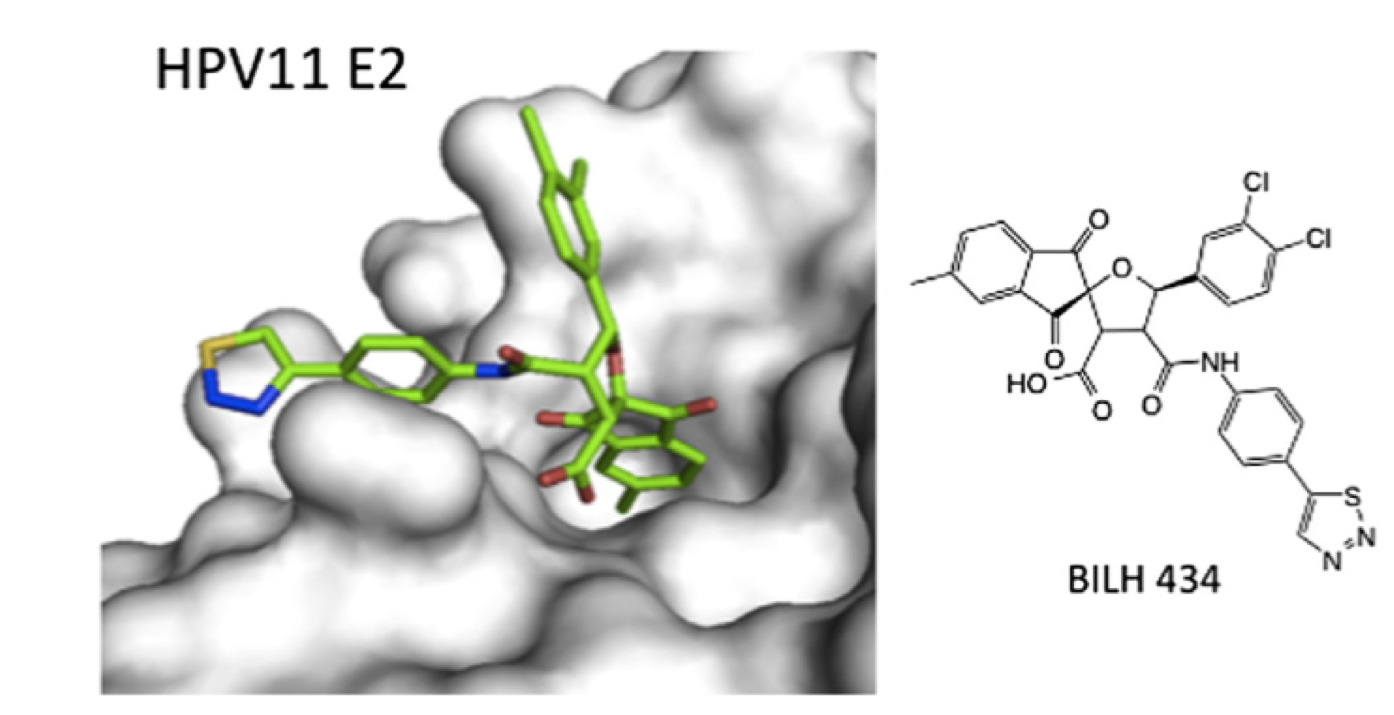
\includegraphics[width=0.7\textwidth]{introDTI}
  \caption{小分子化合物和蛋白质相互作用的示例(摘自Arkin,2014)\cite{arkin2014small}}
  \label{fig:introDTI}
\end{figure}

与此同时,近期的研究表明,即使最初设计为特异性单靶点的小分子药物,也通常会与多种
非预先设计的蛋白质相互结合\cite{hopkins2009drug}(off-target effect,脱靶效应),
即表现出多向药理性(polypharmacology)。药物的多向药理性与药物副作用(side
effect)有重要联系\cite{tatonetti2009predicting}。同时,利用药物的多向药理性,研
究药物的潜在新功能,即药物重定位\cite{ashburn2004drug}(drug repositioning),也
成了近些年药物研究的热点之一\cite{mei2012opportunities}。

目前,已有的药物与蛋白质的相互作用记录还相对较少,存在着很大的探索空间
\cite{keiser2009predicting}。截止2006年3月,美国食品药监局(US Food and Drug
Administration, FDA)批准的小分子治疗药物数目为1,065种
(去除附加物,维生素,前导药物等),其中人源蛋白质靶标数目为394种,平均每个药物约有1.8个
蛋白质靶标\cite{yildirim2007drug}。有研究估计,平均小分子药物应至少会有6个靶标
\cite{mestres2008data}。故预测化合物靶标对药物脱靶效应预测和药物重定位等也有重要
意义。
\begin{figure}[htbp]
  \centering
  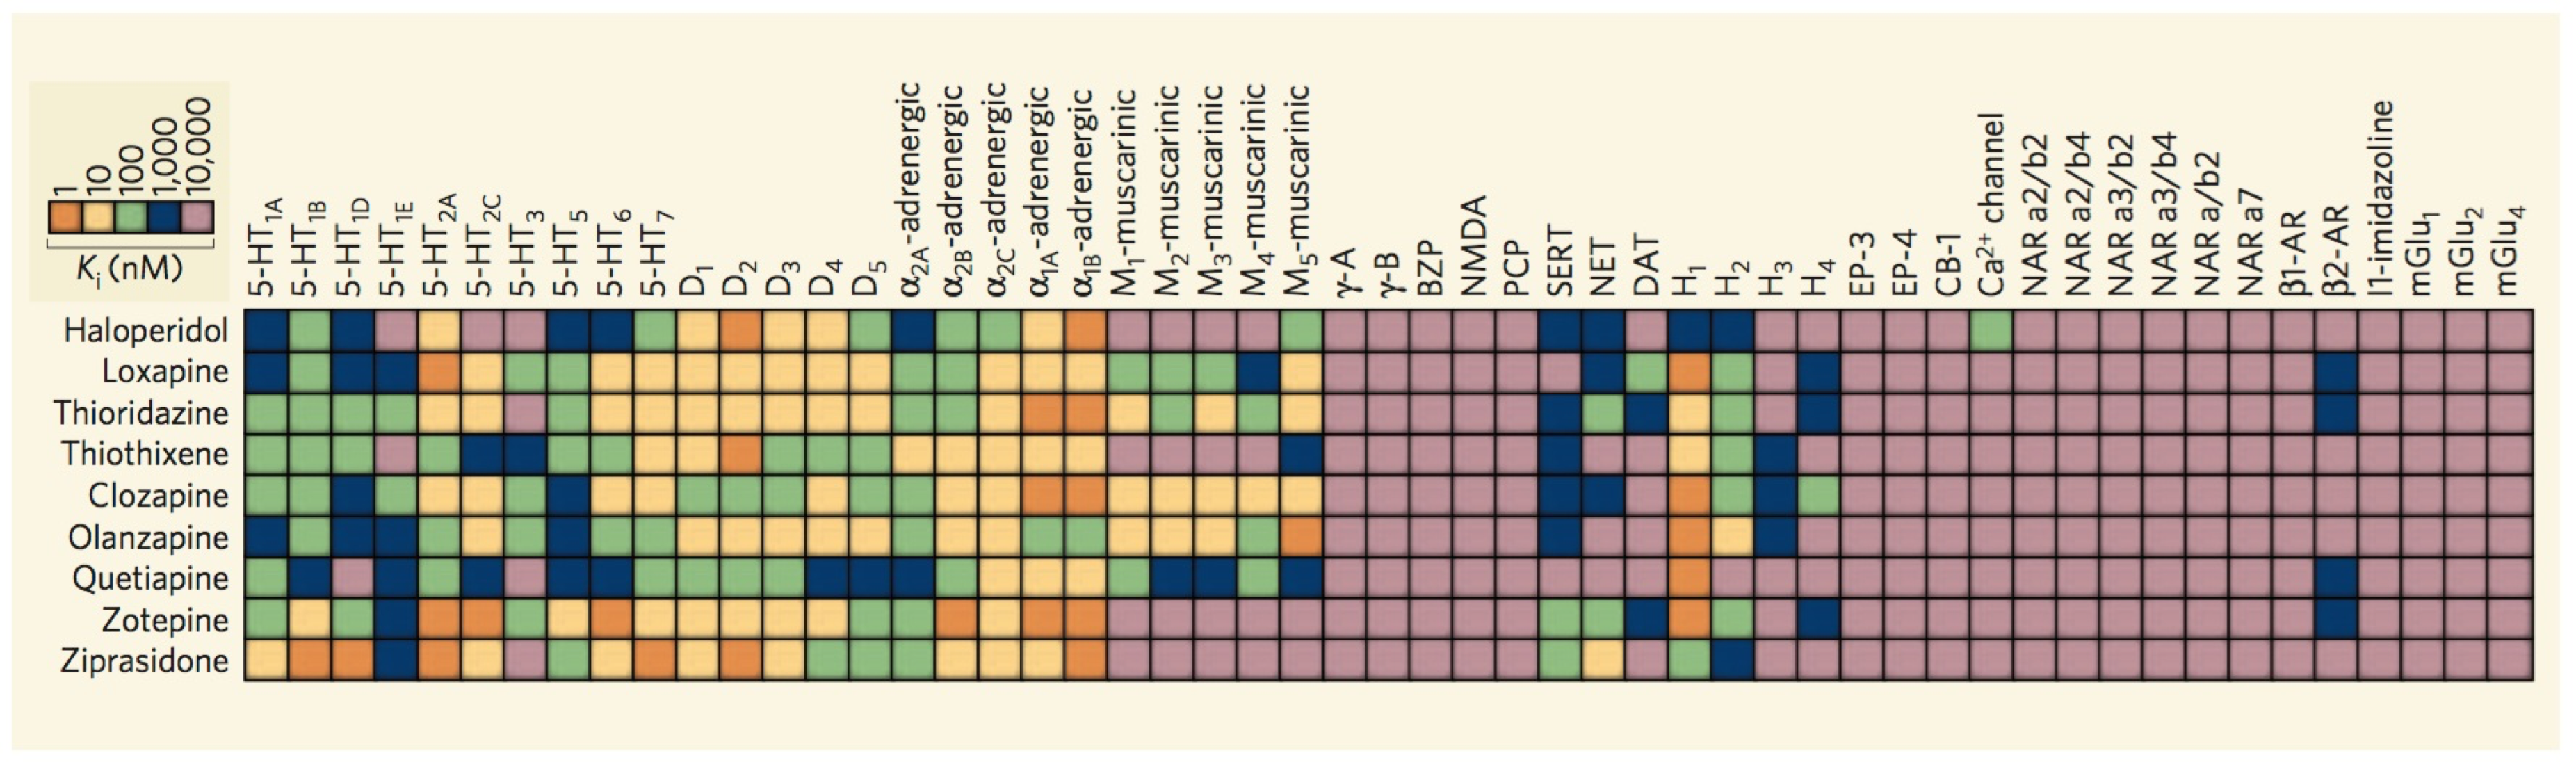
\includegraphics[width=\textwidth]{intorPredictingPromiscuity}
  \caption{单一药物有多靶点的示意(摘自Hopkins, 2009)\cite{hopkins2009drug}。图
    中每一行对应一种药物,每一列对应一种蛋白质。$K_i$值表明二者间的相互作用强度,低的值代表高
    亲和力。}
  \label{fig:introPolypharamacology}
\end{figure}

从实验角度进行化合物靶标验证,存在的主要困难如下。首先,需检测的化合物与蛋白质组
合数目较大。目前主要制药公司收集的活性化合物至少有$10^6$规模
\cite{schenone2013target},而可与化合物结合的蛋白质靶标,尽管具体值还存在争议,
但数目量级在$10^3$尺度\cite{hopkins2002druggable,overington2006many}。其次,药物
靶标检测实验,尤其是高通量筛选(high-throughput screening, HTS),耗时久,成本高
且有一定的数据质量问题\cite{malo2006statistical}。故从计算角度预测化合物靶标,指
导实验设计,是近几年来研究的重点之一。

从计算角度预测化合物靶标,主要有两个大的方向\cite{schenone2013target}。一种是基于蛋白质三维结构的分子对接
(docking)方法,另一种是基于统计模型的化合物靶标预测。

Docking主要利用量子化学等方法,从计算角度,模拟化合物和蛋白质间不同原子
的相互作用。它的优势在于可以清楚地模拟化合物与蛋白质作用时的空间结构或结合模式,但其
计算耗时较长,并且更为重要的是,需要蛋白质有高分辨率的三维晶体结构信息。目前已知
三维结构的蛋白质还相对较少,尤其是细胞膜上的蛋白质,其晶体结构较为难以获取。但已
知的药物中,大约60\%的靶标为膜上蛋白\cite{hopkins2009drug,schenone2013target}。

随着大规模的化合物与蛋白质的数据积累,基于统计模型的化合物靶标预测成为大家关注的
热点\cite{ding2014similarity}。本论文主要研究基于统计模型的化合物预测方法的构建
及应用。在本章的以下部分,我们将对这一方面目前的研究进展进行综述,最后讨论本论文
主要的研究内容和各章节内容安排。
\section{基于统计模型的化合物靶标预测方法研究进展}
\label{sec:methodsum}
总体而言,基于统计模型的化合物靶标预测方法,按照求解问题的分析思路,有以下几种核
心的思想:
\begin{itemize}
\item {\bf 类比法或相似性原则}
  结构或功能相似的化合物倾向于有结构或功能相似的靶标。
\item{\bf 网络模块性或近邻性}
  化合物的靶标在蛋白质相互作用网络或其他构建的网络上有一定的模块性或邻近性。
\item{\bf 特征表示分析}
  通过将化合物或蛋白质进行结构拆分等方式,将其表示为一列特征向量的描述,从而转为
  模式识别或回归分析问题。
\end{itemize}

按照模型构建时,对数据的利用方式不同,我们将其归为两类。一类侧重将一对化合物与蛋
白质关系对作为基本独立单元进行考虑,或二者仅是两类不同的节点。
目前大部分从机器学习角度建模,都是这样来考虑。另一类侧重围绕某一种蛋白质,
对与其结合的化合物集合,进行特征分析,研究者也称之为基于配体的建模
\cite{schenone2013target}(ligand-based approach)。传统药物化学中的构效关系\cite{cherkasov2014qsar}
(structure-activity relationship)模型主要从这个角度考虑问题。按照模型的预测目
的不同,化合物靶标预测也可分为定性预测或定量预测两种类型,前者关注化合物
与蛋白质是或否有相互作用的可能,后者关注化合物与蛋白质的结合强度。

不同的分类方式,主要按照近期该领域研究内容中数据利用特点或者主要的思考方式进行归
纳总结。我们下面主要按照求解问题的分析思路,从三个角度,对目前的基于统计建模的化
合物靶标预测方法进行总结。值得注意的是,不同的分析思路和数据利用方式并非相互独立。
\subsection{基于相似性原则的化合物靶标预测方法}
\label{subsec:similarity}
这类方法主要基于这样的假设:结构或功能相似的药物其作用的蛋白质倾向于相同或相似。
主要的步骤即构建化合物及蛋白质的相似性度量,进而借合适的算法将两种相似性度量,
通过已有的药物与蛋白质相互作用关联起来。
\subsubsection{化合物的相似性的度量}
化合物的相似性可以从结构和表型两个角度定义。

化合物的结构相似性计算,通常利用已有的化学信息学软件,计算其平面(two
dimensions, 2D)或立体(three dimensions, 3D)的结构相似性
\cite{vilar2014similarity}。2D相似性的计算主要是将化合物拆分为不同的子结构
(substructure)有无的位向量(bit vector)表示,称为分子指纹(fingerprints)。利
用位向量间的交与并的比值(Tanimoto coeeficient, TC)值作为相似性度量
(\autoref{fig:introMACCSexam})。3D结构相似性的计算相对较为复杂。其中一类也是
构建3D的子结构表示,如化学药效团(立体和电子云相关的化学特征,是化合物与特定靶点
结合必需位置\cite{yang2010pharmacophore})等,利用TC值作为度量;另一种则指通过空
间构型,静电属性和原子空间位置进行结构比对\cite{dixon2006phase}。
\begin{figure}[htb]
  \centering
  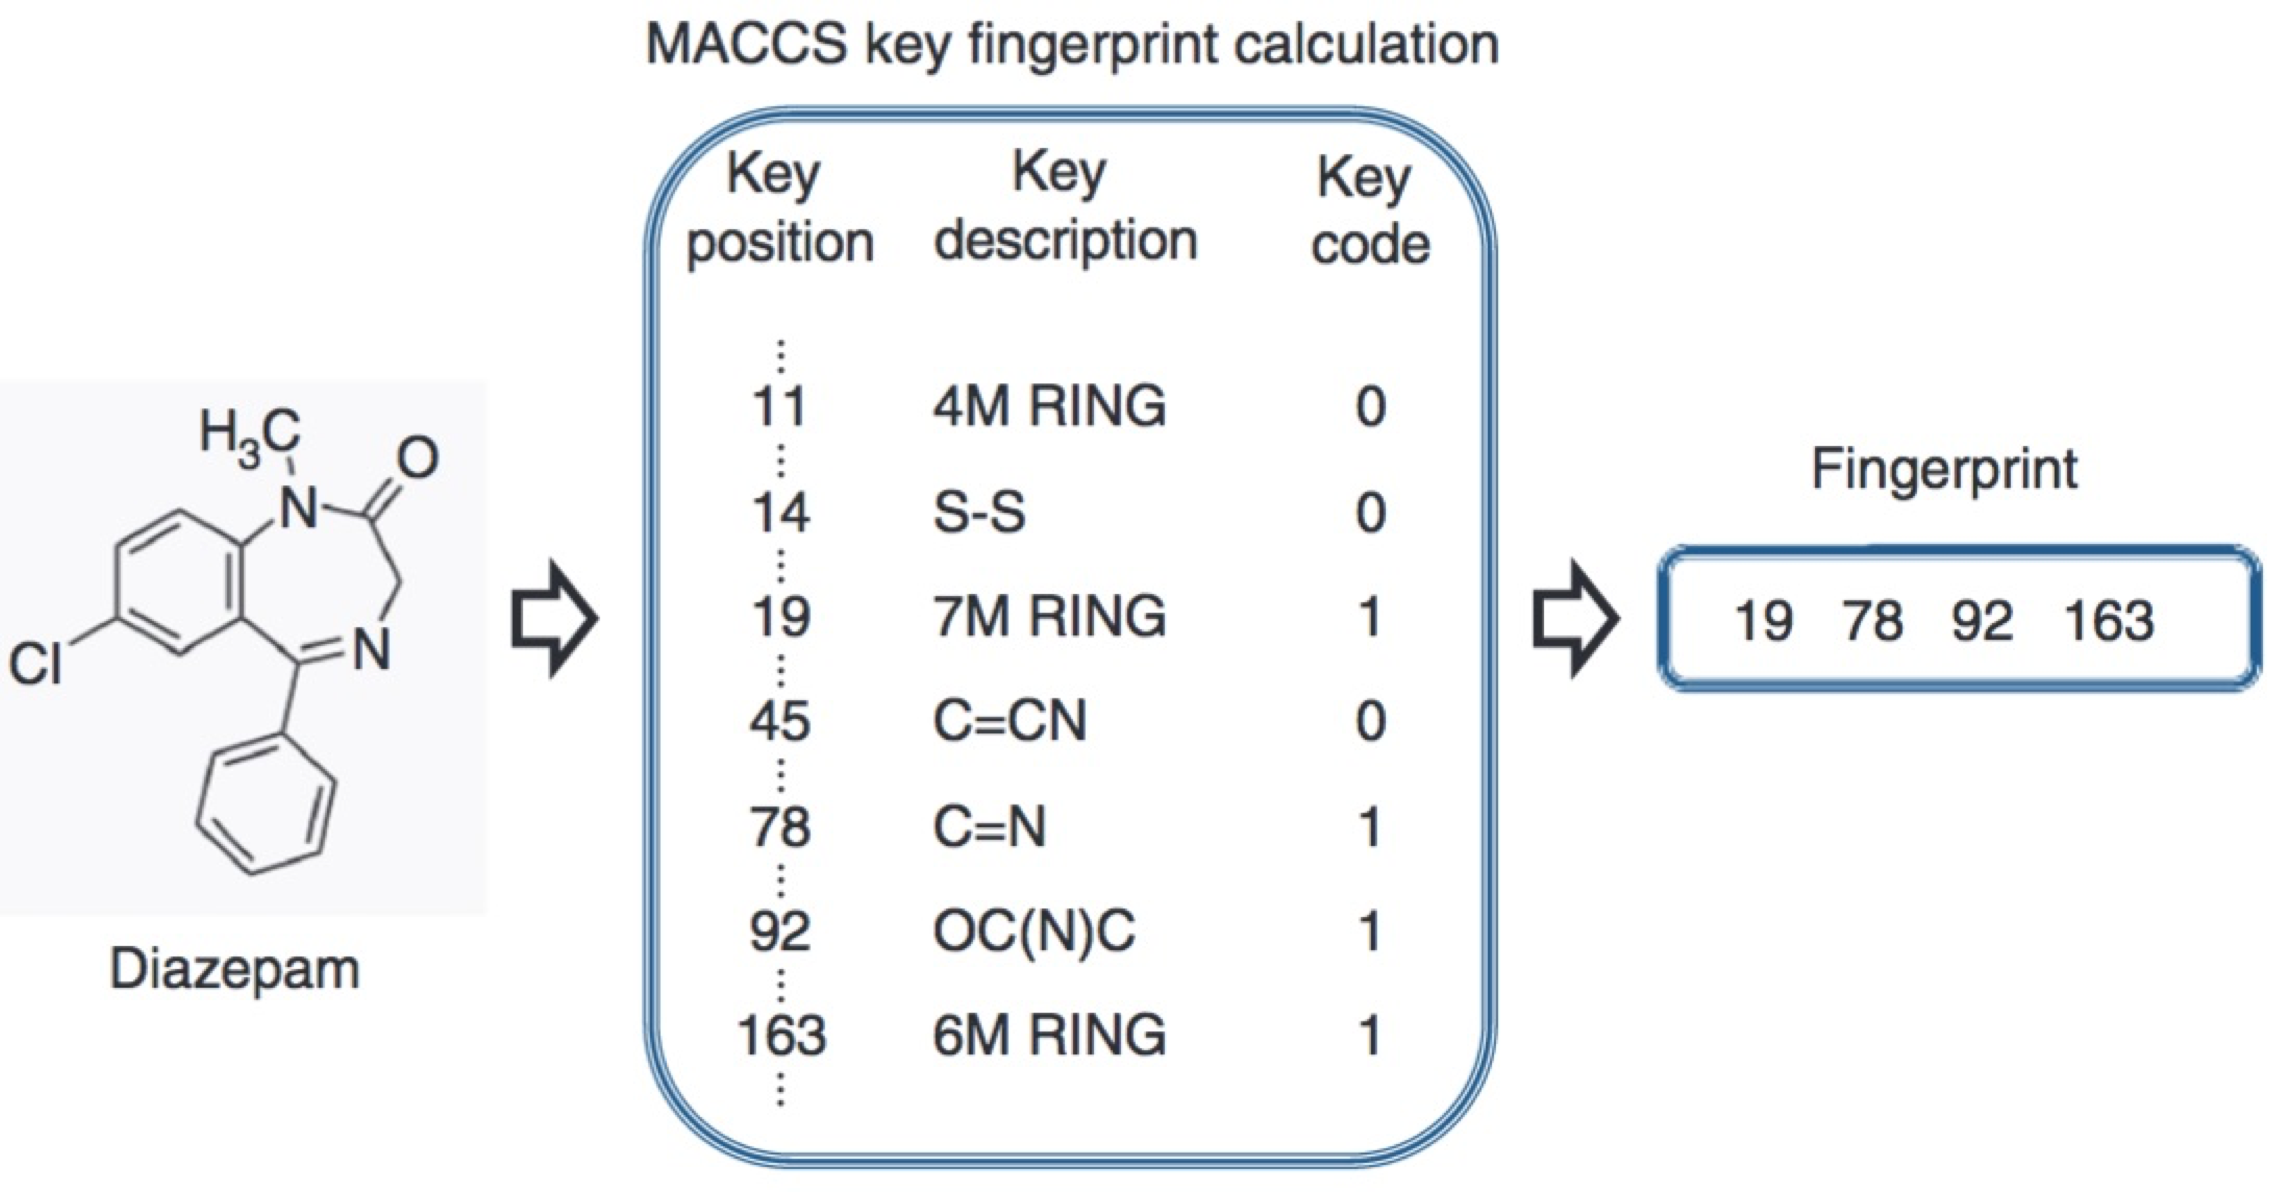
\includegraphics[width=\textwidth]{introMACCSexam}
  \caption{化合物分子指纹表示示例(摘自 Durant,
    2002)\cite{durant2002reoptimization}}
  \label{fig:introMACCSexam}
\end{figure}
\begin{figure}[ht]
  \centering
  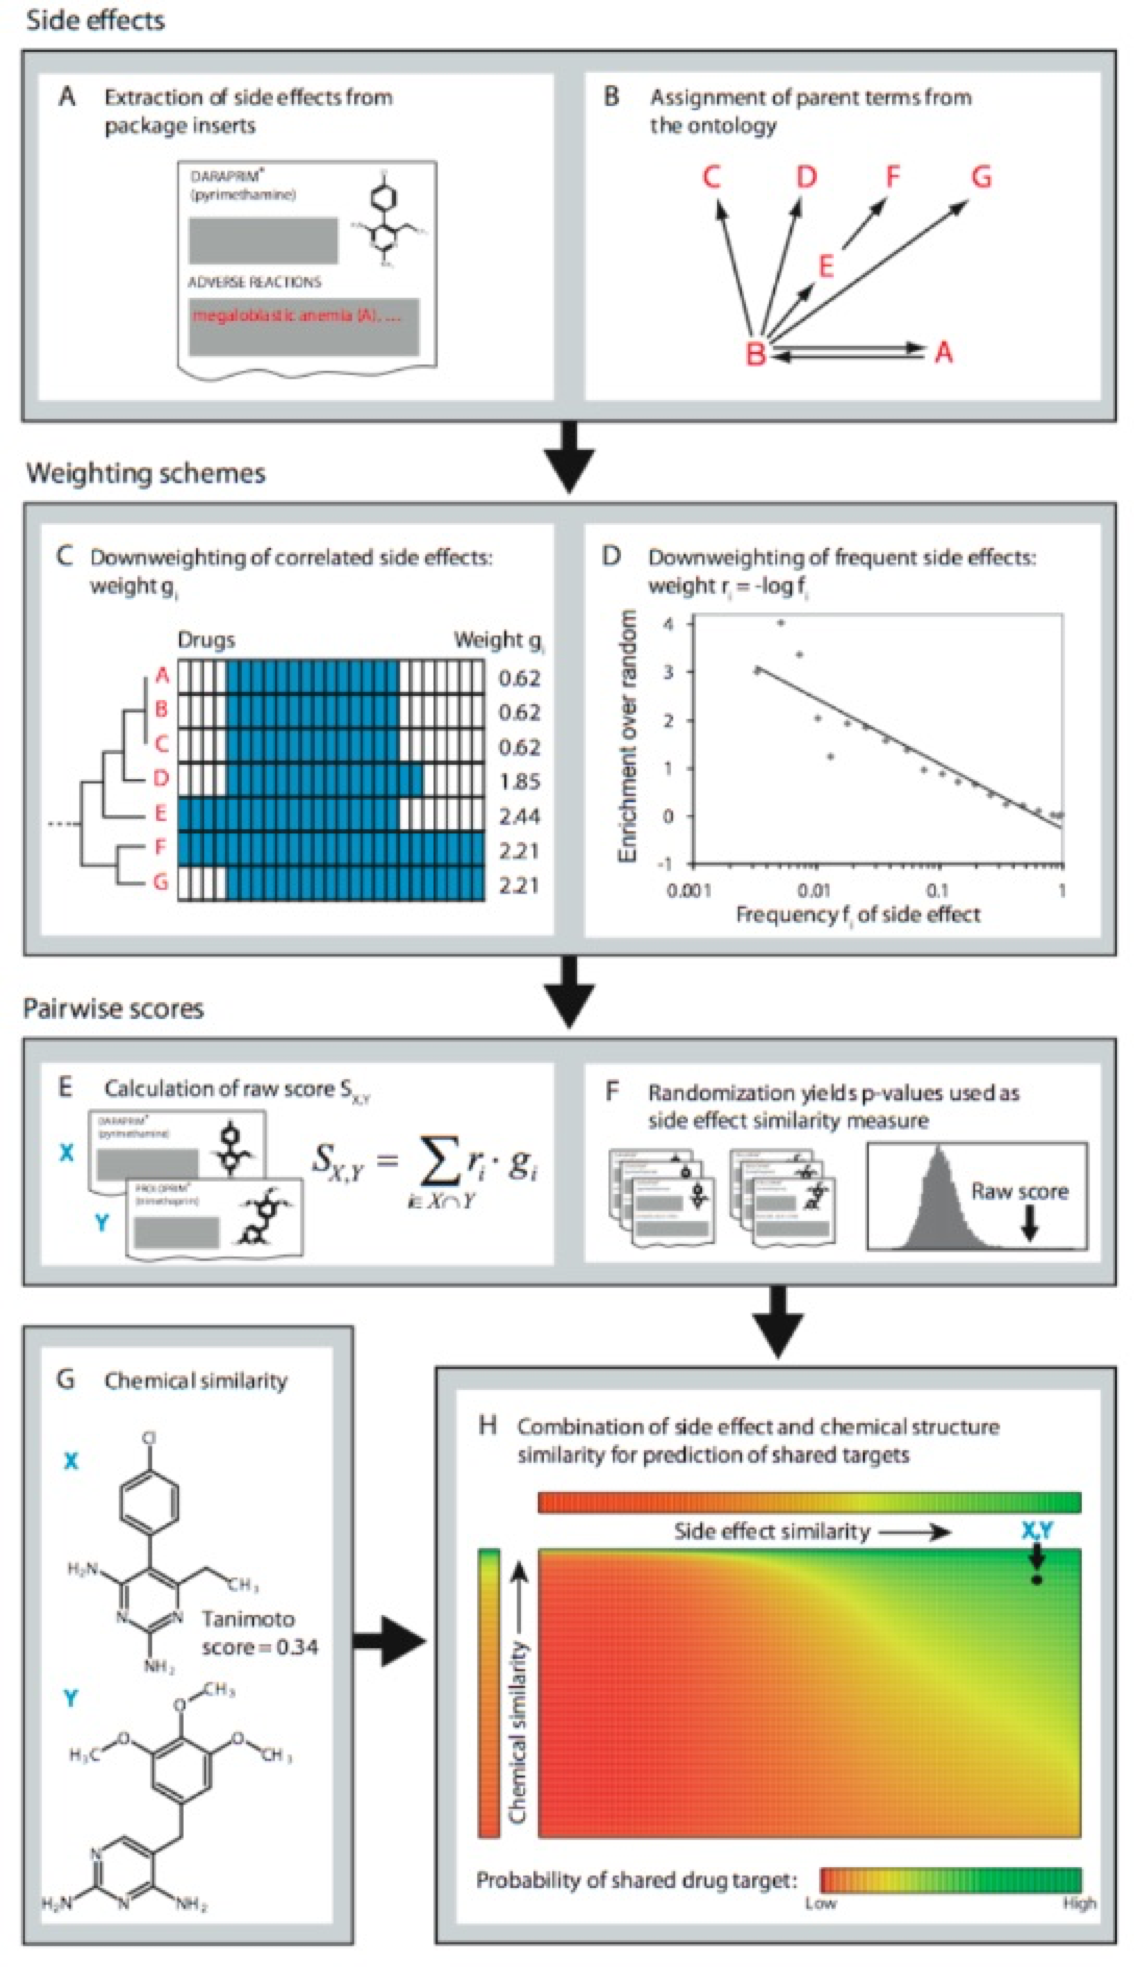
\includegraphics[width=0.7\textwidth]{introSideEffect}
  \caption{利用药物副作用相似性和药物化学结构相似性预测药物靶标(摘自Campillos, 2008)\cite{campillos2008drug}}
  \label{fig:introSideEffect}
\end{figure}
基于表型的相似性度量,主要考虑不同化合物在生物活性等方面体现出的功能相似性。其中,
最有代表性的是通过药物的副作用相似性预测药物靶点
\cite{campillos2008drug}(\autoref{fig:introSideEffect})。作者手工收集药物使
用说明中对药物副作用的介绍,基于此构建药物副作用信息的度量,结合药物结构相似性,预
测药物靶标。后续工作中,他们构建了药物副作用记录的数据库\cite{kuhn2015sider}。
同时,也有若干组采用药物副作用进行药物靶点预测\cite{takarabe2012drug,
  cheng2013prediction}。

表型信息相似性还可以依据药物疗效,如利用药物组织学疗效信息编码系统(Anatomic
Therapeutic Chemical, ATC)\cite{gottlieb2011predict,zhao2010network},或
基于化合物处理后的细胞表达谱数据(gene expression profiles)的相似性数据
\cite{wang2013prediction}等方式定义
(\autoref{fig:introGeneExp})。如近年来研究者们公布的 Connectivity Map (CMAP)数
据集,记录了大规模的小分子化合物干扰后的人类细胞的表达谱数据
\cite{lamb2006connectivity}; LINCS (Library of Integrated Cellular Signatures)
数据集\footnote{Broad Institute Library of Integrated Cellular
Signatures (LINCS) \url{http://www.lincscloud.org/}}, 也称为下一代CMAP。
\begin{figure}[htb]
  \centering
  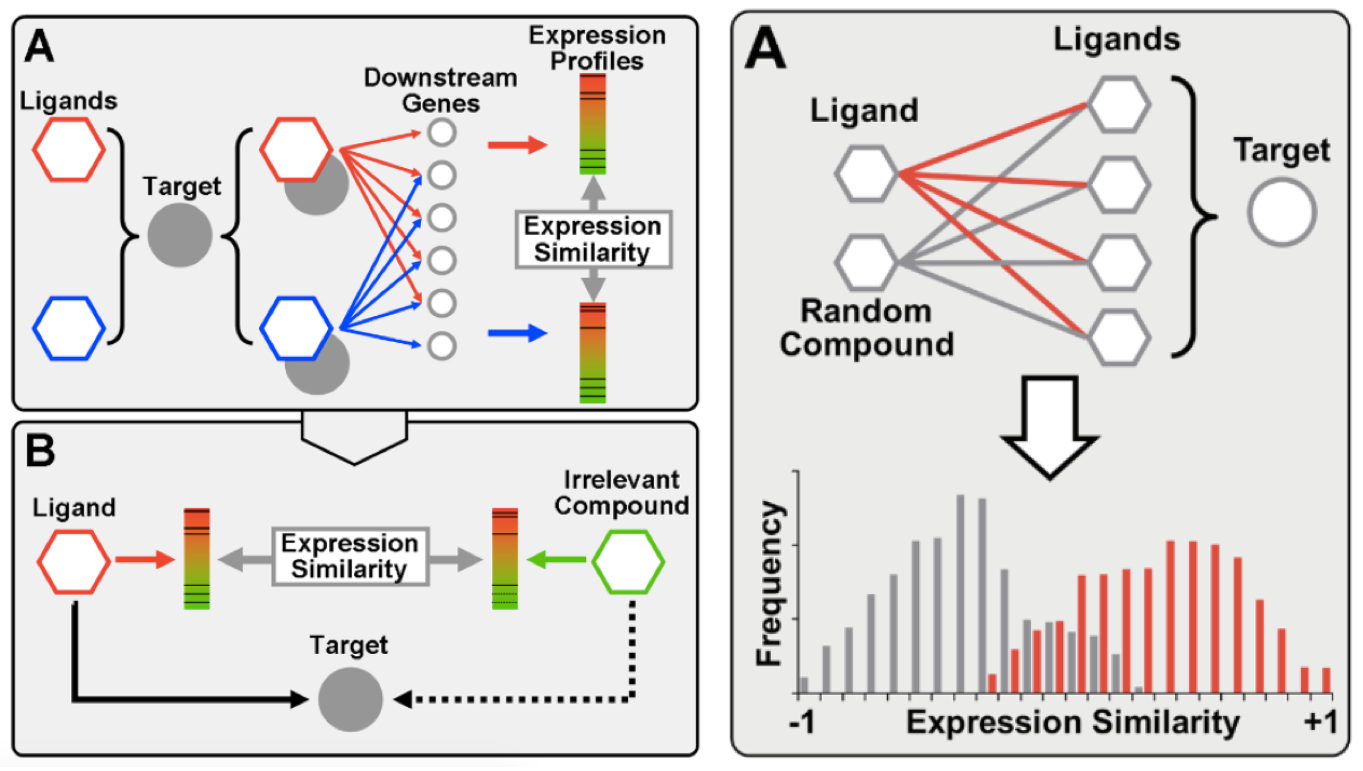
\includegraphics[width=\textwidth]{introGeneExp}
  \caption{基于化合物对应的细胞表达谱相似性进行靶点预测(摘自Wang, 2013)\cite{wang2013prediction}}
  \label{fig:introGeneExp}
\end{figure}

显然,我们如果能从多个角度对化合物进行相似性度量,就会获取更多的相似信息,从而有
更好的预测准确率。但是在实际中,很多化合物都缺少相关的表达谱数据,治疗信息等,从
而有一定的数据缺失。故如果我们的方法基于多种角度的相似性度量,则其在研究新型化合
物的表现上就会受到很大的约束。
\subsubsection{蛋白质的相似性度量}
蛋白质的相似性度量,主要通过其氨基酸序列相似性,或者其包括的结构域(protein
domain),蛋白质相互作用网络间的距离远近,蛋白质特异性特征等信息进行度量。蛋白质的结构域是构成蛋白
质的结构和功能的单元,化合物与蛋白质的相互作用,主要是通过与蛋白质的结构域进行结
合\cite{bateman2004pfam,overington2006many}。

这方面比较新颖的工作是Keiser等人提出的相似度集合方法(similarity ensemble
approach, SEA)\cite{keiser2007relating}。SEA方法是一种基于配体的方法。它通过蛋
白质对应的配体(与蛋白质相互作用的化合物)集合间的化学结构相似性定量地估计蛋白质
间的药理活性相似性。
\begin{figure}[htbp] \centering
  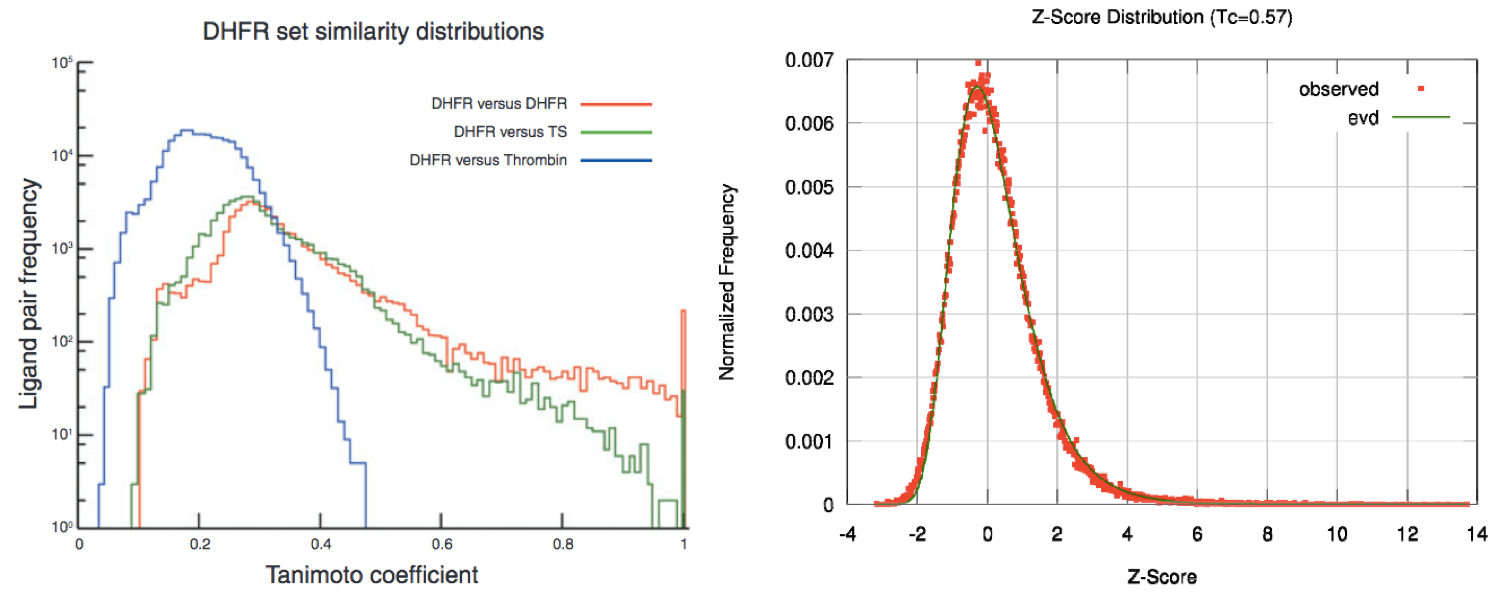
\includegraphics[width=\textwidth]{introSEA}
  \caption{SEA方法示例(摘自Keiser,2007)\cite{keiser2007relating}。左图为不同
蛋白质对应的的配体间结构相似性的分数经验分布;右图拟合随机情况下蛋白质对应配体的
结构相似性分数累加后经过正则化处理服从极值分布。}
  \label{fig:introSEA}
\end{figure}

该方法的核心思想在于利用与蛋白质相互作用的小分子化合物集合来代表该蛋白质在药理方
面的性质。从而,当我们判断给定药物或者小分子化合物是否与某一蛋白质相互作用时,我
们只需要考虑该小分子化合物和这个蛋白质对应的化合物集合的整体相似度。通过观察随机
组合的化合物集合间化学结构相似度分数(该分数可以近似地理解为两个集合间两两化合物
化学结构相似度之和)在归一化后服从极值分布(Extreme Value Distribution)这一现象
\cite{hosking1985estimation}(\autoref{fig:introSEA})。类比
BLAST\cite{altschul1997gapped}原理,在衡量化合物集合之间整体相似度时,利用
BLAST中用到的E-value描述其相似度分数的统计显著性。两个蛋白质间若打分的统计显著性
高,说明它们存在药理相似性;而给定化合物与某一蛋白质对应的化合物间打分的统计显著
性高,则暗示了该化合物有可能与给定的蛋白质相互作用。

研究者利用实验验证了部分预测结果。后续中,他们利用该方法,对已有药物的新靶点以及
已有药物对70多种给定的副作用相关蛋白质的相互作用进行大规模预测和实验验证
\cite{keiser2009predicting,lounkine2012large}。

总体而言,SEA方法有较高的准确率,但是其受限制于蛋白质需要有较多
配体记录信息,并偏向于化学结构保守的化合物预测,对于发现新结构类型的化合
物方面存在一定的不足\cite{yabuuchi2011analysis}。
\subsubsection{关联化学相似性空间与蛋白质相似性空间}
在产生化合物的相似性矩阵和蛋白质的相似性矩阵后,一系列的统计学习模型发展出来,通
过已有的化合物和蛋白质相互作用数据,将不同空间的信息关联起来。最直接的方法为近邻
法(nearest neighbor, NN)\cite{bleakley2009supervised},该方法直接简洁,计算相
对快速。进一步,我们可以将化合物和蛋白质的相互作用看做二分图(bipartite graph),
从而利用局部二分方法(bipartite local method, BLM)将原预测二分图边的问题转化为
有监督的机器学习问题
\cite{bleakley2007supervised,bleakley2009supervised,mordelet2008sirene}。这里面
主要技巧在于支持向量机(support vector machine, SVM)等一类机器学习方法,在模型
训练中只依赖于与样本间相似性定义的核函数\cite{suykens1999least}(kernel
function),当针对某一对蛋白质和化合物是否相互作用时,我们可以固定一方,如该蛋白
质。此时通过将对应的化合物与该蛋白质的是否有连边,将化合物打上两种标签,进而在化
合物空间中利用SVM等方法进行模型训练。这类方法劣势在于同时需要训练多种分类器,而
且每种分类器的正样本(即连边数目)数据有限。成对核函数方法\cite{jacob2008protein}(Pairwise kernel
method, PKM)做了改良,直接将一对化合物与蛋白质作为训练的样本,有无连边作为标签,
通过定义不同对化合物与蛋白质间的整体相似性,利用核函数进行建模。这样,只需要一种
预测模型即可。同时,研究者通过对药物和蛋白质投影到低维空间,在低维空间中计算化合
物与蛋白质的相互作用分数\cite{gonen2012predicting},该作用分数可以通过投
影矩阵与给定的两种相似性矩阵直接表达。这也可以看做是核函数思想的一种拓展。

Ding等
人\cite{ding2014similarity}对基于相似性的机器学习方法进行了综合的讨论与计算结果
比较,不同的方法在不同实验条件下,表现优劣各异。Ding等同时指出,近些年药物设计中
从已有药物出发,通过有限地结构修饰,可能会导致基于相似性的预测方法评价中表现得过
于良好。
\subsection{基于网络模块性的化合物靶标预测方法}
系统生物学的发展,让人们对药物的多药理性有了更深入的认识\cite{pei2014systems}。
从生物网络的角度,理解药物作用机理和作用靶点,即“网络药理学”的观念,逐渐得重
视\cite{hopkins2008network}。通过构建药物与蛋白质相互作用的二分网络,Yildirim等人
\cite{yildirim2007drug}发现大部分药物在该网络中形成较大的连接度高的模块
(\autoref{fig:introDTnetwork})。在890个药物中有788个药物存在和其他药物共享同一
靶标的现象,而这其中最大的连接子网有476个药物。
\begin{figure}[htb]
  \centering
  \includegraphics[width=\textwidth]{introDTN_DTnetwork}
  \caption{药物与蛋白质的二分网络(摘自Yildirim,2007)\cite{yildirim2007drug}}
  \label{fig:introDTnetwork}
\end{figure}

直接利用药物和蛋白质的二分网络,Cheng等人\cite{cheng2012prediction}构建了基于网
络拓扑结构的扩散模型(\autoref{fig:introNBI})。计算结果表明,该模优于他们直接依
赖化合物结构相似性或蛋白质序列相似性的近邻法。直接在二分网络上的建模,思路简洁清
晰,但存在的不足在于不能对不在该网络的药物或者蛋白质进行靶点预测。这一定程度上限
制了我们对该模型的应用范围。
\begin{figure}[htb]
  \centering
  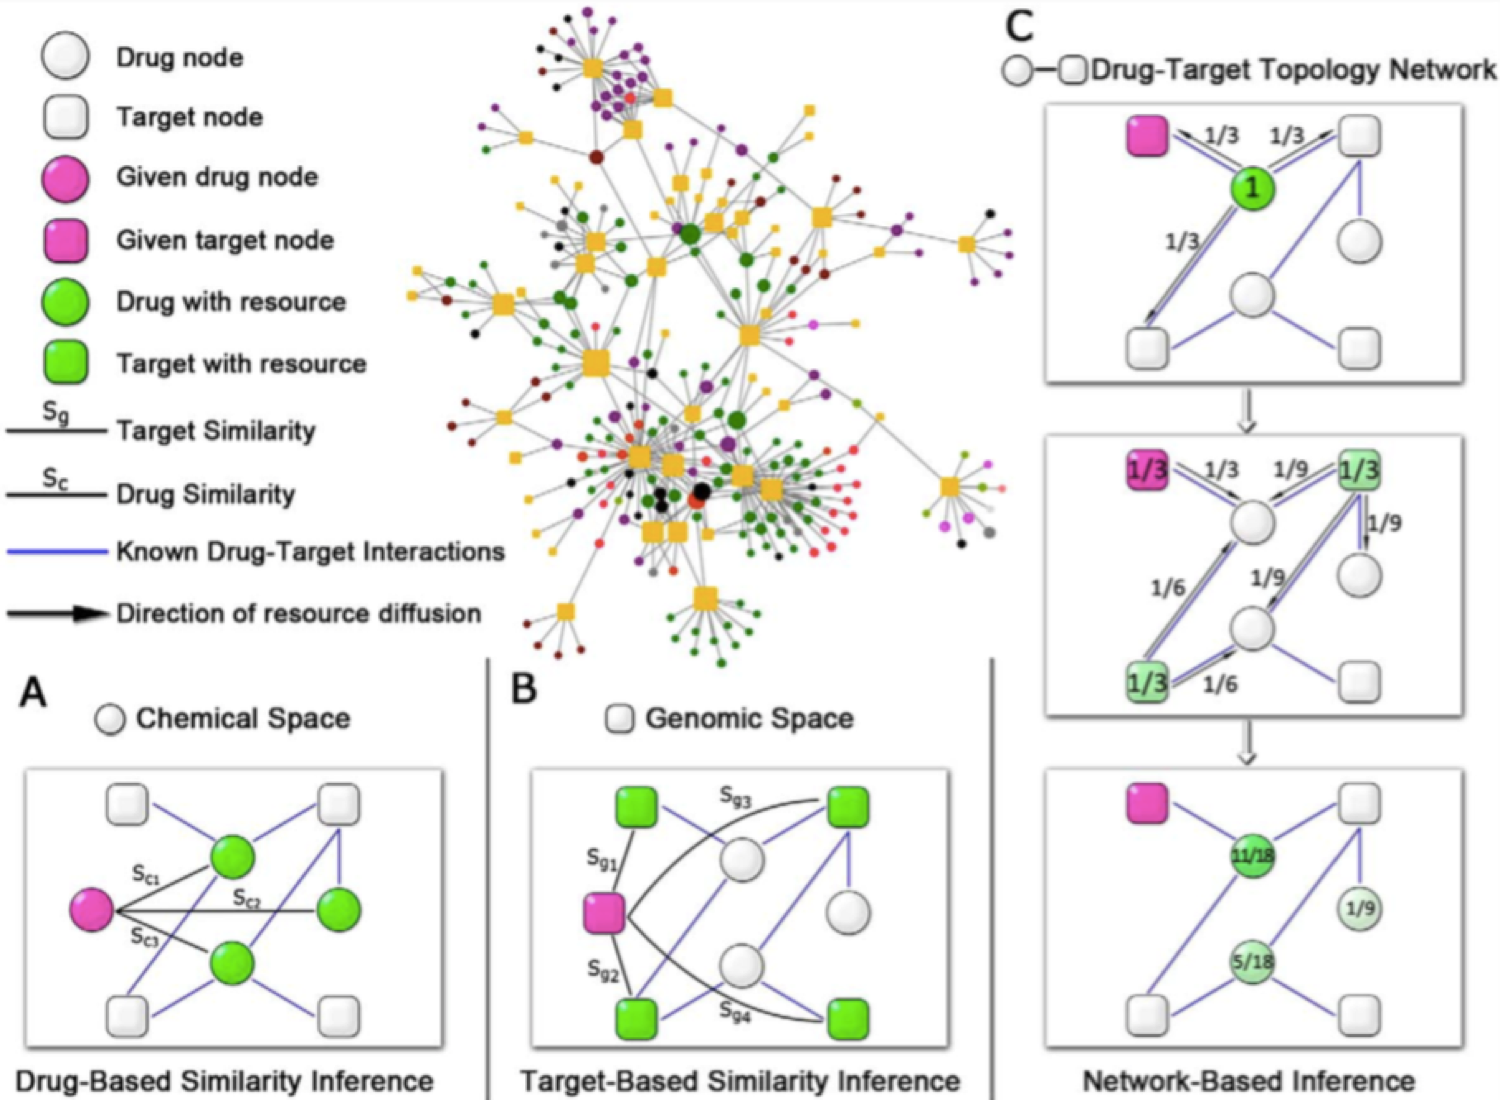
\includegraphics[width=\textwidth]{introNBI}
  \caption{基于药物与蛋白质的二分网络的网络推断方法(摘自Cheng, 2012)\cite{cheng2013prediction}}
  \label{fig:introNBI}
\end{figure}

除了上述二分网络,构建异质性的化合物和蛋白质双层网络,在此基础上,利用回
归模型进行化合物靶标预测的方法DrugCIPHER\cite{zhao2010network} 也表现出了优秀的
预测能力,得到广泛的认可\cite{barabasi2011network}。研究者观察到化学结构相似或疗
效相似的药物,对应的蛋白质靶标在蛋白质相互作用(protein-protein interaction, PPI)
网络上距离较近(\autoref{fig:introDrugCIPHER}),呈现出一定的网络模块性
(modularity)。同时,将疗效相似性与化学结构相似性联合考虑,对模型预测性能有较好
的提升。
\begin{figure}[htb]
  \centering
  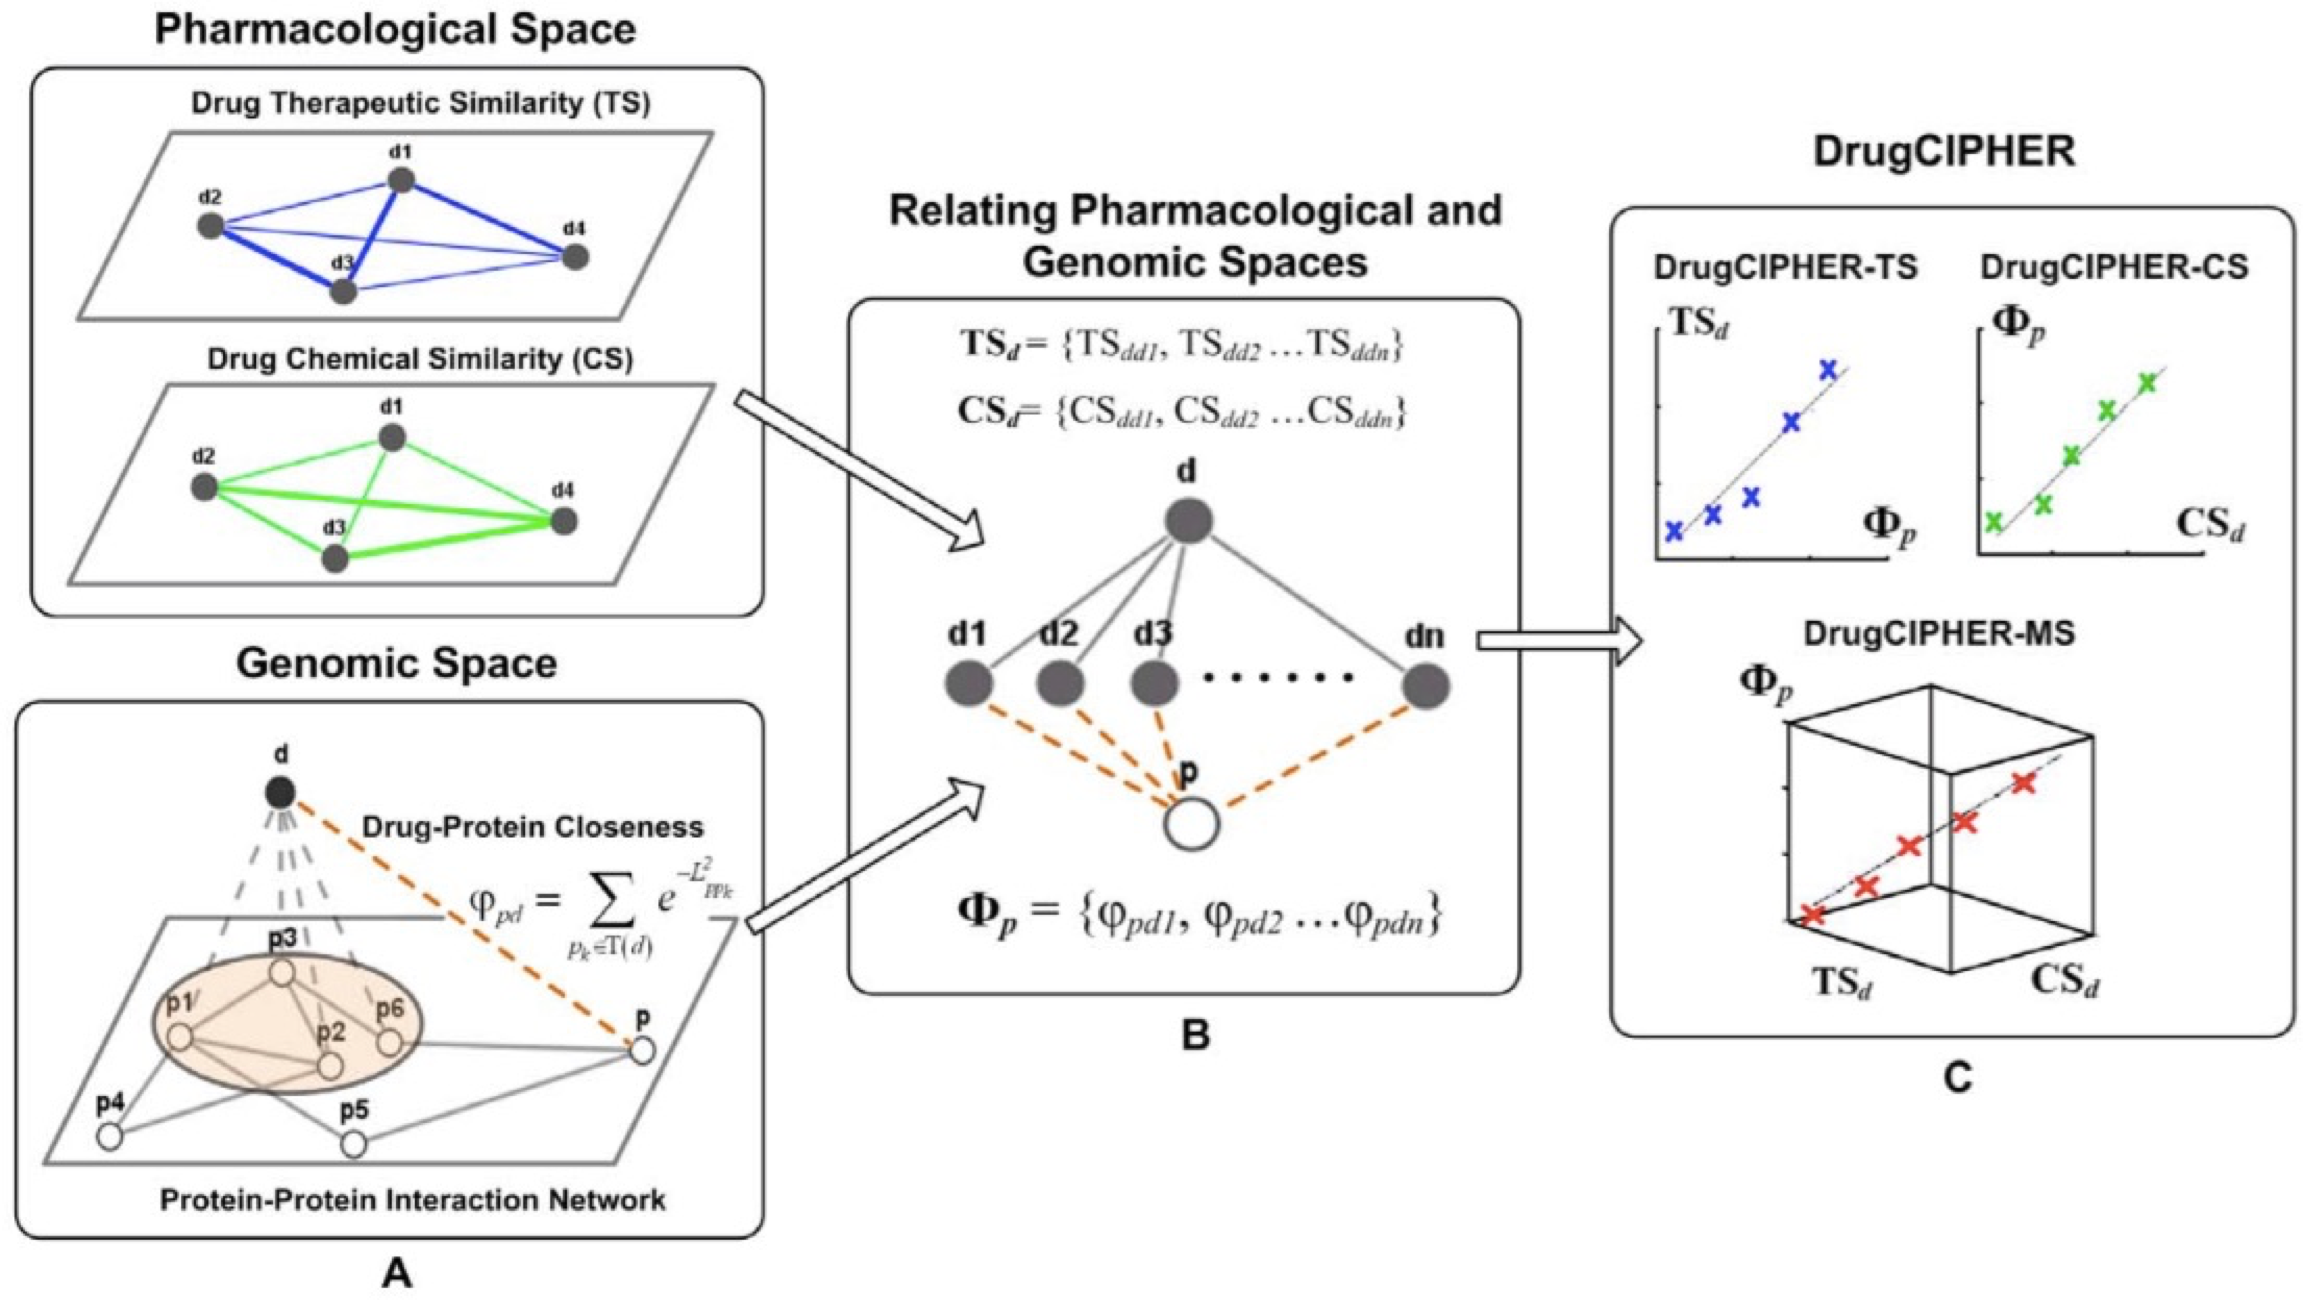
\includegraphics[width=\textwidth]{introDrugCIPHER}
  \caption{DrugCIPHER示意图(摘自Zhao, 2010)\cite{zhao2010network}}
  \label{fig:introDrugCIPHER}
\end{figure}

基于网络的化合物靶标模型打开了一扇门,使得很多计算机科学或数学中,基于图及网络的
算法有了应用的领域,如随机游走(random walk)模型
\cite{seal2015optimizing,yao2011modularity}, 网络检索时网页排名的算法
\cite{zhang2015drug}(如Page Rank算法),网络最大流算法\cite{chen2011uncover}等。

网络
模型的核心思想实际为一类典型关联分析\cite{wang2014drug}(guilt by association,
GBA),与近几年从网络角度预测疾病的关联基因等有异曲同工之处
\cite{lee2011prioritizing}。DrugCIPHER方法即受益于基于网络推断致病基因的方法
CIPHER\cite{wu2008network}的启发。值得注意的一点是,网络分析方法相较于直接靶点的
推断,更侧重于效应靶点的预测,即药物通过网络信息可以影响到的蛋白质。
\subsection{基于特征表示的化合物靶标预测方法}
在章节\ref{subsec:similarity}中,计算化合物或蛋白质的结构相似性,主要基于提取
不同的子结构或序列等特征,构成特征表示向量,进而进行整体的相似性评估,如化合物可
以利用2D分子指纹表示,蛋白质可以利用其所含有的结构域表示。直接利用这些特征表示,
进行模式识别或回归分析等,是基于特征表示的化合物靶标预测方法的基本思路
(\autoref{fig:introChemoinformatics})。
\begin{figure}[htb]
  \centering
  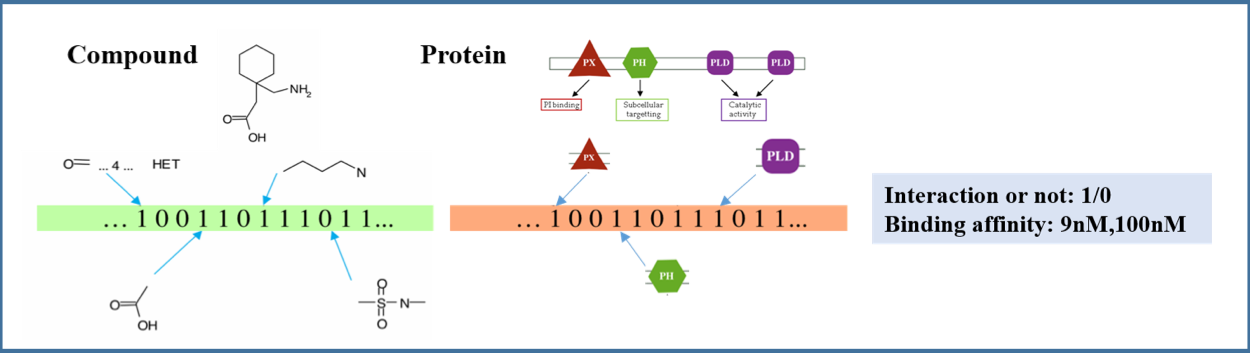
\includegraphics[width=\textwidth]{introChemoinformatics}
  \caption{基于特征表示的化合物靶标预测方法示意。}
  \label{fig:introChemoinformatics}
\end{figure}

Yabuuchi等人\cite{yabuuchi2011analysis}收集了GPCR家族和激酶(Kinase)家族的蛋白
质与化合物相互作用的数据。通过提取化合物的结构特征和蛋白质的氨基酸序列特征,将每
对化合物与蛋白质利用上述特征表示,并作为一个样本,利用SVM算法进行化合物靶标预测。
同部分已知三维结构的蛋白质进行基于结构的分子对接模型,基于配体的计算模型(见章节
\ref{sec:methodsum})以及实验测试等角度,该模型都表现出了较好的性能。同时,该模
型可以有效地预测出新的骨架迁越\cite{sun2012classification}(scaffold-hopping)的
化合物。Scaffold-hopping主要指化合物能达到与先前化合物同等的生物活性等功效,但拥
有新的结构骨架。

进一步,Besnard等人\cite{besnard2012automated}收集了ChEMBL数据库
\cite{bento2014chembl}记录的化合物与蛋白质结合强度的数据,共133,061种化合物,
215,967个活性数据。利用拉普拉斯形式修饰的朴素贝叶斯模型
\cite{xia2004classification,rogers2005using}(Laplacian-modified naive Bayeisan
model),对784种蛋白质构建了相应的基于配体的化合物靶标预测模型。与以往研究思路不
同,他们利用这些模型,协助他们进行虚拟化合物合成。从某一化合物结构出发,通过罗列
该化合物结构上的多种修饰,对虚拟的修饰后的化合物利用上述模型进行靶点预测等,如此
找到期望的化合物结构。

上述方法的逆向思考,即从已知的化合物和蛋白质相互作用数据中,估计化合物化学子结构与蛋
白质结构域等的相互作用逐渐受到重视
\cite{yamanishi2011extracting,duran2013analysis,duran2014chemo}。这类特征可以用
来估计化合物靶标,也可用来分析其中的关键化学子结构。通常可以利用费歇尔检验
(Fisher test)或模式识别中的特征贡献度分析等(\autoref{fig:introDuran})。
\begin{figure}[htb]
  \centering
  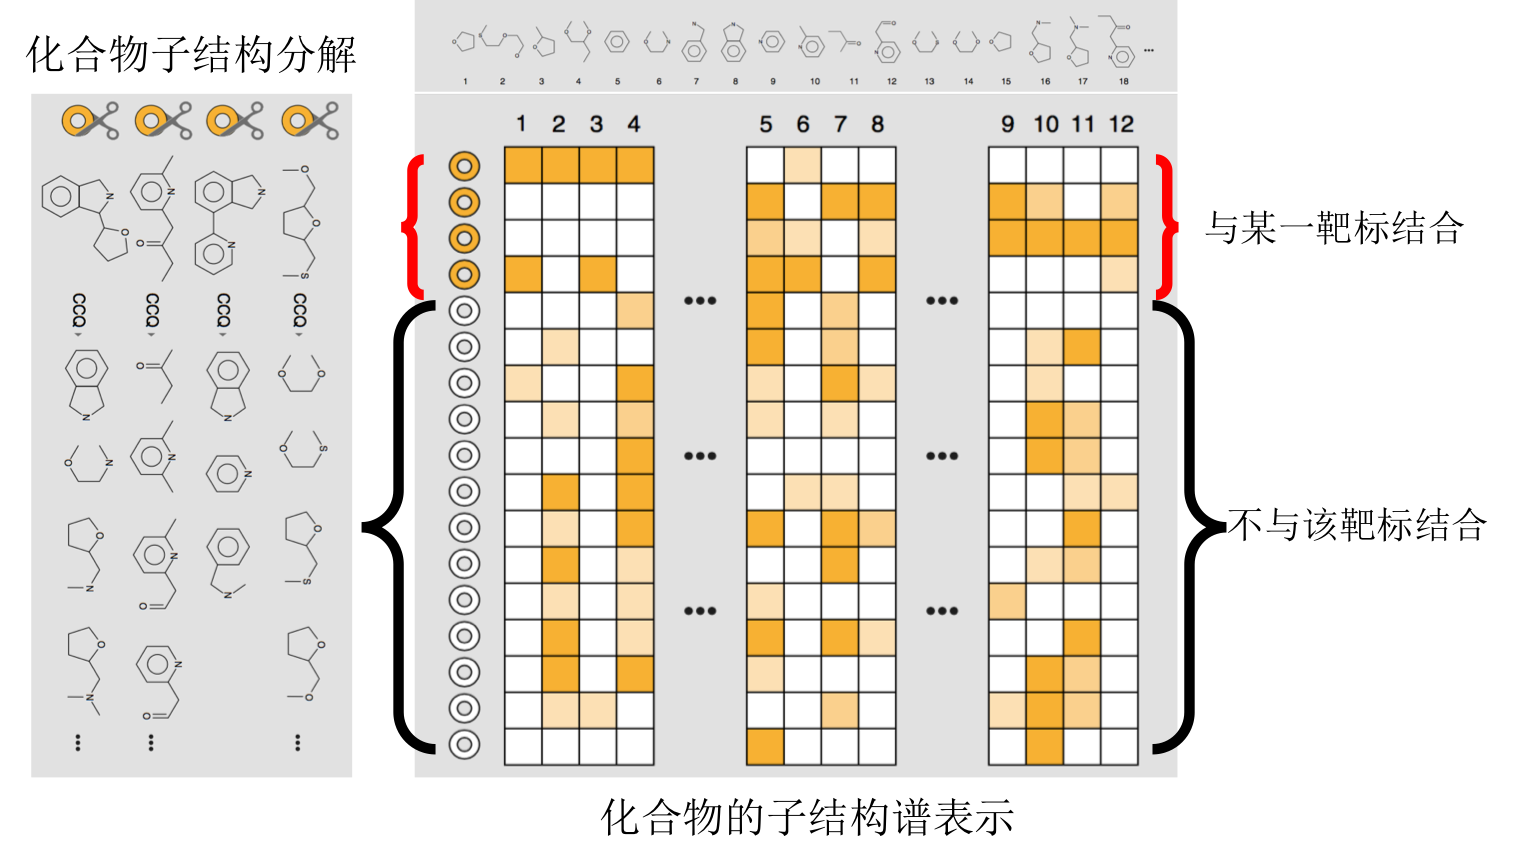
\includegraphics[width=\textwidth]{introChemoinformatics-1}
  \caption{从已知的化合物靶标数据中,估计关键的化学子结构}
  \label{fig:introDuran}
\end{figure}

作为QSAR问题的子问题之一,基于特征表示的化合物靶标预测方法,强调了化合物与蛋白质相
互作用的机制,即它们子结构间的相互作用,从而该类方法拥有相对更好的模型在生物化学
方面的解释能力,可以与实验紧密结合。同时,这类基于特征表示的建模,可以推广到药物
在体内吸收,分布,代谢,排除和毒性(absorption, distribution, metabolism,
excretion, and toxicity, ADMET)等方面的建模\cite{shen2010estimation,cheng2013prediction}。

以上我们从相似性原则,网络模块性原则和特征表示等三方面总结了目前基于统计模型的化
合物靶标预测方法,并分析了不同分析角度的优势和不足。其中部分方法同时考虑了不同出
发角度,如DrugCIPHER整合了相似性和网络模块性两方面的信息。近期的方法也重视从多角
度出发,如将多种相似性信息统一到一个联合模型
\cite{gottlieb2011predict,wu2014integrating},整合化学信息学和网络方面的信息
\cite{wu2016sdtnbi},或整合多种机器学习模型的预测结果\cite{yuan2016druge}等。值
得注意的是,化合物与蛋白质的相互作用有多种类型,如化合物激活或抑制蛋白质的活性,
即作用的方向性等。Wang等人利用限制玻尔兹曼机(restricted Boltzmann machine, RBM),
在前述的二分网络中,将网络边注释了多种化合物与蛋白质间结合类型,进而在该多维度网
络上,预测化合物与蛋白质的作用类型\cite{yang2014drug}。
\section{模型的计算验证方法}
\subsection{负样本数据的构建}
负样本信息,即明确的化合物与蛋白质不会发生相互作用,对于定性预测化合物靶标方法的
模型训练,以及对于定性和定量方法的模型验证等非常重要。然而,文献数据库中通常不
会将化合物与蛋白质相互作用的阴性结果报道出来,从而我们没有明确的负样本信息。目前
主要的化合物靶标预测方法,负样本的选取都是从没有报道的化合物与蛋白质对中,随机抽
取\cite{ding2014similarity}。从统计角度,尽管化合物与蛋白质间未知的相互作用数目较
多,但相比较二者的组合空间而言,数量是稀疏的,故随机抽取一定数目的负样本是合理的。

Liu等人\cite{liu2015improving}巧妙地利用相似性原理,从已有的化合物靶标记录出发,将化合物与相应的靶
标不相似的蛋白质作为负样本。计算表明,高质量的负样本数据,在传统的方法上取得了一
定的性能提高。
\subsection{交叉验证}
交叉验证(cross validation, CV)是机器学习常用的检测模型表现能力的方法\cite{friedman2001elements}。其主
要的思路为将我们观测到的样本随机均匀分为若干等分,通常采样三等份,五等份或十等份,
对应着三倍,五倍和十倍交叉验证。模型训练时,依次抽取其中一份作为测试集,剩余的作
为训练集。利用训练集得到的模型,观测在测试集上的表现,如功效曲线(receiver
operator characteristic curve, ROC curve)下的面积(area under roc curve, AUC),
均方错误率(mean square error)等。相对极端的情形是,每次抽取一个样本作为测试样本,
称之为留一验证(leave one out, LOO)。

在化合物靶标预测中,不同方法利用的交叉验证方式或数据集通常不同。目前这方面的比较
还缺少统一的数据集合,对预测结果的解释也不能都以AUC为主,还需要考虑跟多的生物学
证据,以及特征的生物学解释\cite{liu2015improving}。Pahikkala等人
\cite{pahikkala2014toward}讨论了化合物靶标预测时,需要考虑到测试集中的化合物或蛋
白质是否在训练集中都出现,或都没有出现,或有一方出现,这些都更接近真实的化合靶点
预测问题。
\section{化合物靶标相关的数据库介绍}
目前,关于化合物靶标记录方面,主要的数据库库有BindingDB数据库
\cite{liu2007bindingdb}, DrugBank数据库\cite{wishart2008drugbank},KEGG数据库
\cite{kanehisa2000kegg},STITCH数据库\cite{kuhn2008stitch},欧洲生物信息学中心
(European Bioinformatics Institute, EBI)维护的ChEMBL数据库
\cite{bento2014chembl}和美国国家生物技术信息中心(National Center of
Biotechnology Information, NCBI)维护的PubChem数据库\cite{wang2009pubchem}等。

BindingDB数据库主要记录小分子化合物与蛋白质作用强度的数据,目前含有6,487种蛋白质,
554,532种小分子化合物,共1,254,324个结合数据记录。其中,共有5,861个化合物与蛋白质
相互结合的晶体数据(蛋白质序列相似性在85\%以上),在蛋白质序
列相似性100\%条件下有2,291个数据。

DrugBank数据库主要记录药物相关的信息,目前含有8232种药物,其中2004个FDA审批通过
的小分子药物,221种FDA审批通过的蛋白质或多肽类药物,93种如维生素等的营养物质和超
过6,000个实验药物。每种药物都会记录其靶标,物化性质,药物疗效分类等200多条信息。

KEGG数据库全称为基因与基因组东京百科全书(Kyoto Encyclopedia of Genes and
Genomes),里面关于蛋白质全面的信息,同时KEGG DRUG, KEGG COMPOUND 记录了药物,化
合物方面的一些信息。

STITCH数据库记录并预测了一部分化合物与蛋白质相互作用的数据,其中含有300,000种化
合物,来自1,133种物种的共200多万个蛋白质。

ChEMBL数据库主要记录具有成药性的活性小分子化合物信息,数据为人工从主要文献中检索
而来,注释了化合物ADMET,功能等多方面信息。目前含有2,936,512种化合物,11,224种蛋
白质,活性数据条目为14,371,219个(不完全针对蛋白质,有细胞层次等)。

PubChem数据库主要收集小分子化合物(不限于是否有成药性)的信息,并含有多种生物活
性数据记录。活性数据主要来自40多个组织,如美国政府机构,美国国家卫生研究所
(National Institute of Health, NIH)资助的筛选中心,以及
药厂和主要实验室。该数据库提供如聚类,化学相似
性计算,化学子结构特征等多种工具。目前包含的化合物数目不少于92,000,000种,活性数
据至少有1,200,000个。这些活性数据中记录的靶标蛋白质数目约为5,000种。注意,ChEMBL
数据库已包含部分PubChem中的数据。

\section{本文的主要工作和结构安排}
本文工作围绕从统计模型角度,构建预测化合物靶标的计算方法。通过提取化合物的子结构
与物理化学信息,蛋白质结构域和序列相似性信息等,对化合物及蛋白质进行特征表示,
结合已有的大规模化合物与蛋白质相互作用数据,从定性及定量模型两个角度研究该问题。

第一章为引言部分,介绍了化合物靶标预测问题的背景及意义。并对基于统计模型的化
合物靶标预测方面进行文献综述。提出了本论文主要研究的具体目标和研究手段。

药物与蛋白质的相互作用主要取决于它们子结构之间的相互作用。之前在这方面的研究,主
要是独立地考虑不同子结构对在药物与蛋白质结合中的贡献度,而忽视了它们之间互相影响
的因素。论文的第二章,我们从全局优化的角度,在已有的药物靶标数据中,估计药物子结
构与蛋白质结构域相互作用的信息,并以此给出一种定性预测化合物靶标的模型。全局优化
在这里的含义是同时考虑不同的药物子结构与蛋白质结构域对间的相互影响关系,从而综合
地评估不同子结构对的贡献。

在定性模型的基础上,论文的第三章,我们对定量化合物靶标预测模型进行了深入研究。以
往的研究方法,通常会单独地对某一蛋白质相互作用的化合物集合进行模型构建,或者直接对与一
组蛋白质相应的化合物集合进行模型构建(单任务学习方式)。前者忽略了不同蛋白质之间可能具有的药理活性
相似性,后者忽视了不同蛋白质之间的特异性。通过观测到同一蛋白质家族中,序列相似的蛋
白质其药理活性相似的特点,我们构建了基于层次贝叶斯框架的多任务学习模型,从而可以更为
充分地利用观测数据。

论文的第四章,我们利用GIFT方法构建了与蛋白质或蛋白质结构域存在明显相关性的化学子
结构靶标库。在此基础上,分析化学子结构与蛋白质结构域的二分网络特点。同时,我们利
用ML-2DQSAR方法构建了G蛋白偶联受体家族和激酶家族共273个蛋白质族对应的化学子结构
特征谱系。最后,我们针对一类重要的中药小分子化合物银杏内酯,进行靶点预测。银杏内
酯有多个化学结构较为相似的成分,不同成分间既有共同的生物活性,又存在一定的不同。
传统的基于化学结构相似性的分析方法,在探究它们活性机制上存在一定的困难。故我们利
用化学子结构拆分的方法,研究它们子结构的差异带来的靶标预测结果的不同。

在论文的第五章中,我们对论文工作的创新性成果进行总结,并对该方向的研究方向进行一
定的讨论和展望。